% Based on docs/ambiguities/template.tex. Retain this decision history.
\documentclass[a4paper,12pt]{article}
\usepackage[margin=19mm]{geometry}
\usepackage{amsmath,amssymb,graphicx,xcolor}
\usepackage{fontspec}
\usepackage{xepersian}
\settextfont{XB Roya}
\setlatintextfont{Latin Modern Roman}
\definecolor{ink}{HTML}{173D75}
\graphicspath{{images/}}
\setlength{\parindent}{0pt}
\setlength{\parskip}{5pt}
\linespread{1.12}
\newcommand{\qtitle}[2]{{\Large\bfseries\color{ink} پرسش \lr{#1}: #2}\par}
\newcommand{\answer}{\par\medskip\textbf{پاسخ ریاضی برای بازبینی بعدی و تاریخ:}\par\vspace{15mm}\hrule\medskip}
\begin{document}
{\LARGE\bfseries پرسش‌های ابهام جلسهٔ \lr{08}}\par
{\large جزوهٔ جبر پیشرفتهٔ دکتر خسروی}\par
شمارهٔ صفحه‌ها، شمارهٔ یک‌مبنای صفحه در فایل پی‌دی‌اف است، نه شمارهٔ دست‌نویس.
پرسش حل‌نشده هنوز در اسلایدها به‌عنوان نتیجهٔ قطعی اثبات پذیرفته نشده است.
\medskip\hrule\medskip

\qtitle{L08-Q01}{گام پایانی جهت عکس خاصیت جهانی جمع مستقیم}
\textbf{وضعیت:} باز برای بازبینی بعدی؛ تکمیل اثبات به تعویق افتاده است.
ثبت در تاریخ \lr{2026-10-25}.\par
\textbf{نشانی منبع:} نسخهٔ \lr{primary}، صفحهٔ \lr{5}، بالای صفحه تا خط افقی؛
ساخت نگاشت‌ها در نیمهٔ پایین صفحهٔ \lr{4} آمده است.
\begin{LTR}\small\verb|sources/lectures/08  direct sum.pdf|\end{LTR}
\begin{center}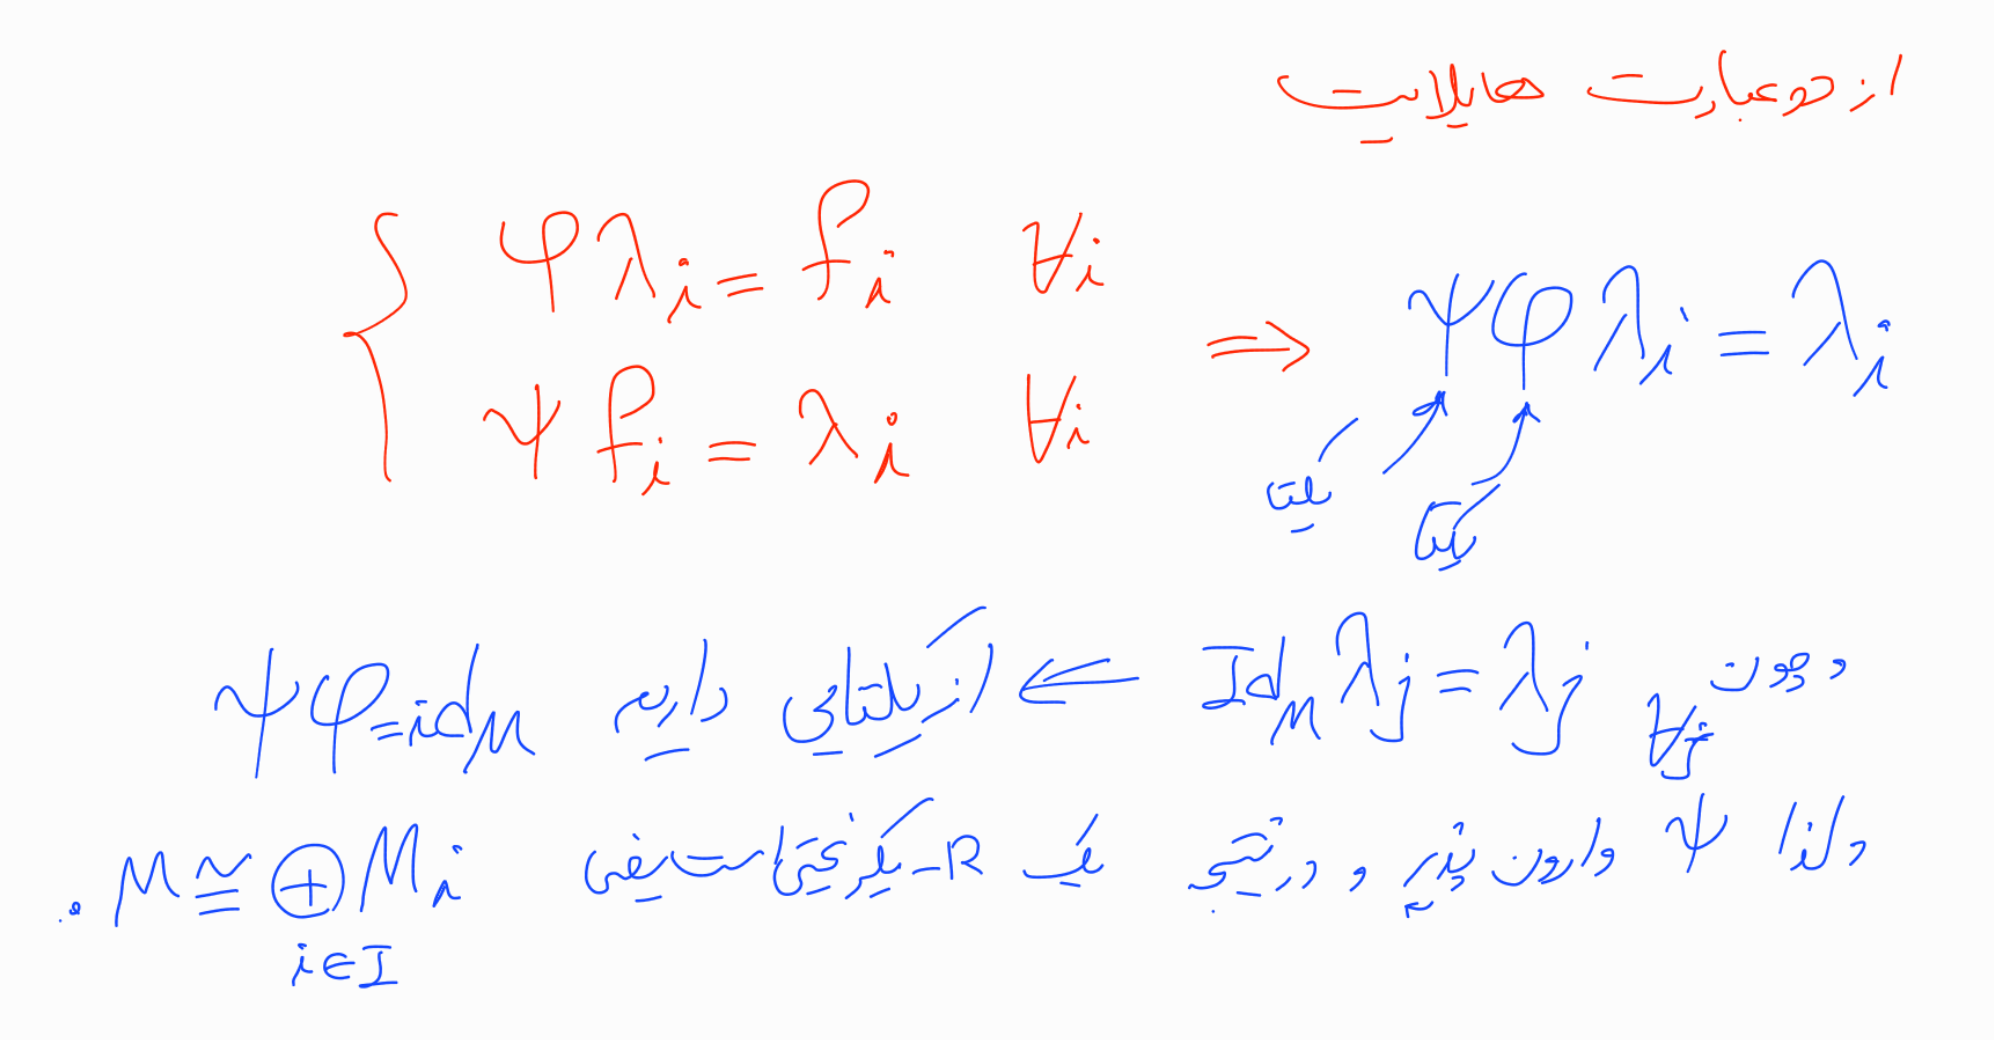
\includegraphics[width=.88\linewidth]{reverse-proof-gap.png}\end{center}
\textbf{عبارت منبع:}
از $\varphi\lambda_i=f_i$ و $\psi f_i=\lambda_i$، به کمک یکتایی،
$\psi\varphi=\operatorname{id}_M$ به دست آمده؛ سپس نوشته شده است که
$\psi$ وارون‌پذیر است و $M\cong\bigoplus_{i\in I}M_i$.

\textbf{دلیل پرسش و دو صورت ممکن:}
این همانی به‌تنهایی وارون‌پذیری را نتیجه نمی‌دهد.
می‌توان افتادگیِ یک گام را در نظر گرفت و با
$X=\bigoplus_{i\in I}M_i$، از
$(\varphi\psi)f_i=f_i$ و یکتایی برای $X$، همانیِ دوم
$\varphi\psi=\operatorname{id}_X$ را افزود؛ یا متن را با ذکر صریحِ ناتمام‌بودن این گام نگه داشت.
افزودن همانی دوم، تکمیل اثباتِ منبع است و هنوز تأیید نشده است.

\textbf{پرسش:} آیا تأیید می‌کنید که گام دومِ پیشنهادی به اسلایدهای اثبات افزوده شود؟
اگر صورت دیگری مدنظر است، لطفاً آن را مشخص کنید.
اسلاید مرتبط: \lr{lec08:reverse-inverse-pending}.
\par\textbf{دستور کاربر در تاریخ \lr{2026-10-25}:} \lr{put in questions PDF}.
پرسش در این سند برای بازبینی بعدی نگه داشته می‌شود؛ این دستور تأییدِ تکمیل پیشنهادی اثبات نیست.
\answer
\end{document}
